\documentclass[12pt, twoside]{article}
\usepackage[letterpaper, margin=1in, headsep=0.5in]{geometry}
\usepackage[english]{babel}
\usepackage[utf8]{inputenc}
\usepackage{amsmath}
\usepackage{amsfonts}
\usepackage{amssymb}
\usepackage{tikz}
\usetikzlibrary{quotes, angles}
\usepackage{graphicx}
\usepackage{enumitem}
\usepackage{multicol}

\newif\ifmeta
\metatrue %print standards and topics tags

\title{Regents Geometry}
\author{Chris Huson}
\date{September 2020}

\usepackage{fancyhdr}
\pagestyle{fancy}
\fancyhf{}
\renewcommand{\headrulewidth}{0pt} % disable the underline of the header
\raggedbottom


\fancyhead[LE]{\thepage}
\fancyhead[RO]{\thepage \\ Name: \hspace{4cm} \,\\}
\fancyhead[LO]{BECA / Dr. Huson / Geometry \\* 1-4 Number line, lengths}

\begin{document}

\subsubsection*{I can work with a number line}
\begin{enumerate}
\item Do Now: Given point $B$ is the midpoint of $\overline{AC}$, with $AB=x+2$, $BC=11$. \\[0.3cm]
    First write and equation representing the situation, then find $x$.\\[0.3cm]
      %\begin{center}
        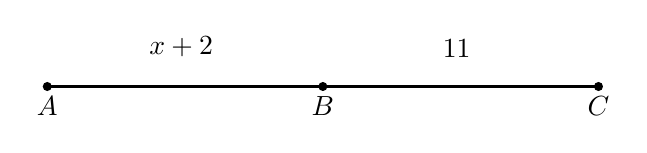
\begin{tikzpicture}
          \draw [fill] (0,0) circle [radius=0.05] node[below]{$A$};
          \draw [-, thick] (0,0)--(7,0);
          \draw [fill] (3.5,0) circle [radius=0.05] node[below]{$B$};
          \draw [fill] (7,0) circle [radius=0.05] node[below]{$C$};
          \node at (1.7,0.25) [above]{$x+2$};
          \node at (5.2,0.25) [above]{$11$};
          %\draw [<->, dashed] (0,-1)--(7,-1);
          %\node at (3.5,-1) [below]{$20$};
        \end{tikzpicture}
      %\end{center} 
      \vspace{1cm}

\item Do Now: The points shown are in a straight line, $\overline{XYZ}$. 
\begin{enumerate}
  \item Measure and label the lengths $XY$ and $YZ$ to the nearest centimeter.\\[1.5cm]
    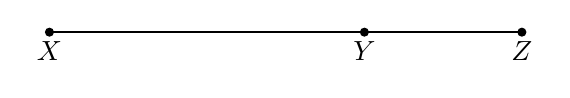
\begin{tikzpicture}
      \draw [-, thick] (1,0)--(7,0);
      \draw [fill] (1,0) circle [radius=0.05] node[below]{$X$};
      \draw [fill] (5,0) circle [radius=0.05] node[below]{$Y$};
      \draw [fill] (7,0) circle [radius=0.05] node[below]{$Z$};
    \end{tikzpicture} \vspace{0.5cm}
  \item Write an equation employing the Segment Addition Postulate.\\ (fill in the blanks with values in centimeters)\\[1cm]
  $XZ=$ \rule{2cm}{0.15mm} $+$ \rule{2cm}{0.15mm} $=$ \rule{2cm}{0.15mm}
\end{enumerate} \vspace{0.5cm}

\item Do Now: Points that are all located on the same plane are $\rule{4cm}{0.15mm}$.

\item Do Now: Write down the name of two line segments shown in the diagram below using proper geometric notation.
  \begin{center}
  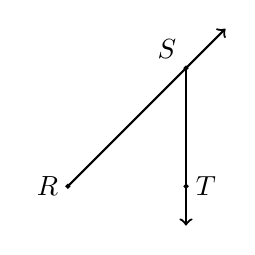
\begin{tikzpicture}[scale=0.5]
    \draw [->, thick] (0,0)--(4,4);
    \draw [->, thick] (3,3)--(3,-1);
    \draw [fill] (0,0) circle [radius=0.05] node[left]{$R$};
    \draw [fill] (3,3) circle [radius=0.05] node[above left]{$S$};
    \draw [fill] (3,0) circle [radius=0.05] node[right]{$T$};
  \end{tikzpicture}
  \end{center}

\item Do Now: Identify two lines in the given plane.\\[0.25in]
    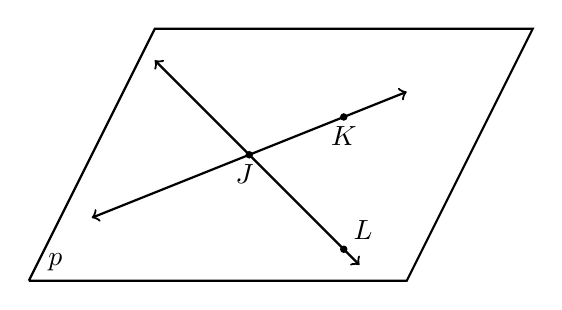
\begin{tikzpicture}[scale=0.8]
      \draw [thick](0,0) node[above right]{$\ p$} --(6,0)--(8,4)--(2,4)--(0,0);
      \draw [<->, thick] (1,1)--(6,3);
      \draw [fill] (3.5,2) circle [radius=0.05] node[below]{$J \ $};
      \draw [fill] (5,2.6) circle [radius=0.05] node[below]{$K$};
      \draw [<->, thick] (2,3.5)--(5.25,.25);
      \draw [fill] (5,0.5) circle [radius=0.05] node[above right]{$L$};
    \end{tikzpicture} %\vspace{2cm}

\newpage
\subsubsection*{Absolute value: the distance from a point to the origin (zero)}
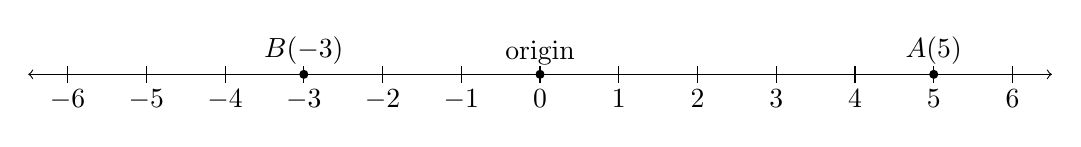
\begin{tikzpicture}
  \draw [<->] (-6.5,0)--(6.5,0);
  \foreach \x in {-6,...,6} %2 leading for diff!=1
    \draw[shift={(\x,0)},color=black] (0pt,-3pt) -- (0pt,3pt) node[below=5pt]  {$\x$};
    \draw [fill] (0,0) circle [radius=0.05] node[above] {origin};
    \draw [fill] (5,0) circle [radius=0.05] node[above] {$A(5)$};
    \draw [fill] (-3,0) circle [radius=0.05] node[above] {$B(-3)$};
\end{tikzpicture} \\[0.5cm]
The absolute value of 5 is 5. $|5|=5$ \\[0.5cm]
The absolute value of $-3$ is 3. $|-3|=3$ \vspace{0.5cm}

\item Find the value of each expression.
\begin{multicols}{2}
  \begin{enumerate}
    \item $|11|=$ \bigskip
    \item $|-7|=$
    \item $|-4.75|=$
    \item $|10-7|=$
  \end{enumerate}
\end{multicols} \vspace{0.5cm}

\item Given $\overleftrightarrow{QS}$ as shown on the number line. \\[20pt] % Midpoint
  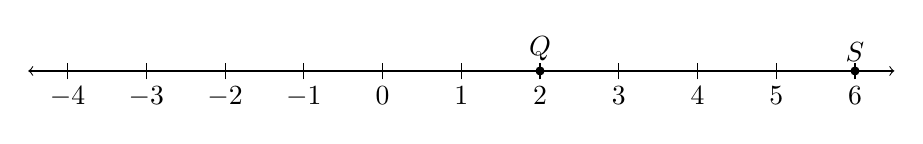
\begin{tikzpicture}
    \draw [<->] (-4.5,0)--(6.5,0);
    \foreach \x in {-4,...,6} %2 leading for diff!=1
      \draw[shift={(\x,0)},color=black] (0pt,-3pt) -- (0pt,3pt) node[below=5pt]  {$\x$};
      \draw [fill] (2,0) circle [radius=0.05] node[above] {$Q$};
      \draw [fill] (6,0) circle [radius=0.05] node[above] {$S$};
  \end{tikzpicture} \bigskip
  \begin{enumerate}
    \item In the given number line units, what is the distance between $Q$ and $S$? \\[0.5cm]
    $QS=$
    \bigskip
    \item Mark the point $R$, the midpoint of $\overline{QS}$.
  \end{enumerate}\vspace{1cm}

\item Given $\overline{MN}$ with $M(-1)$ and $N(3)$, as shown on the number line. \\[0.25cm]
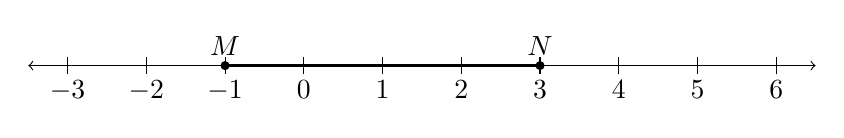
\begin{tikzpicture}
  \draw [<->] (-3.5,0)--(6.5,0);
  \draw [-, thick] (-1,0)--(3,0);
  \foreach \x in {-3,...,6} %2 leading for diff!=1
    \draw[shift={(\x,0)},color=black] (0pt,-3pt) -- (0pt,3pt) node[below=5pt]  {$\x$};
    \draw [fill] (-1,0) circle [radius=0.05] node[above] {$M$};
    \draw [fill] (3,0) circle [radius=0.05] node[above] {$N$};
\end{tikzpicture} \\ \bigskip
What is the length of the segment $\overline{MN}$? Show your work as an equation.\\[1.5cm]
Can a length be a negative number?

\end{enumerate}
\end{document}